% =============================================================================
%  Cifra — Sustentación de Matemáticas Discretas
%  Compilar:  pdflatex presentacion.tex
%  Necesita las carpetas figuras/ y capturas/ al lado de este archivo.
%
%  Para sacar la versión CON notas del presentador, descomentar la línea
%  \setbeameroption{show notes} que está más abajo y volver a compilar.
% =============================================================================
\documentclass[aspectratio=169,10pt]{beamer}

\usepackage[T1]{fontenc}
\usepackage[utf8]{inputenc}
\usepackage{lmodern}
\usepackage{amsmath,amssymb}
\usepackage{booktabs}
\usepackage{graphicx}

% El signo menos "real" (U+2212) y las comillas angulares aparecen en las notas
% del presentador; sin esto pdflatex se queja al compilar la versión con notas.
\DeclareUnicodeCharacter{2212}{-}
\DeclareUnicodeCharacter{00AB}{\guillemotleft}
\DeclareUnicodeCharacter{00BB}{\guillemotright}

% En una instalación normal (Overleaf, TeX Live, MiKTeX) se usa babel en
% español. Si el idioma no está instalado, el documento compila igual.
\IfFileExists{spanish.ldf}{\usepackage[spanish,es-noquoting]{babel}}{}

% --- Notas del presentador ---------------------------------------------------
% Dejar comentado para la versión que se proyecta.
% \setbeameroption{show notes}

% --- Apariencia --------------------------------------------------------------
\usetheme{default}
\usecolortheme{default}
\setbeamertemplate{navigation symbols}{}
\setbeamertemplate{itemize items}[circle]
\setbeamertemplate{caption}{\insertcaption}

% La paleta es la de la aplicación, para que las capturas no se vean pegadas
% de otro sitio.
\definecolor{tinta}{HTML}{0B131A}
\definecolor{tinta2}{HTML}{182027}
\definecolor{apagado}{HTML}{3B434B}
\definecolor{hoja}{HTML}{E5EAEF}
\definecolor{hoja2}{HTML}{C4CBD2}
\definecolor{regla}{HTML}{A1A9AF}
\definecolor{fondo}{HTML}{091017}
\definecolor{fondo2}{HTML}{12191F}
\definecolor{claro}{HTML}{E3E9EE}
\definecolor{claroapagado}{HTML}{9199A1}
\definecolor{acento}{HTML}{970D63}
\definecolor{acentoclaro}{HTML}{E068A6}

\setbeamercolor{normal text}{fg=tinta2,bg=hoja}
\setbeamercolor{structure}{fg=acento}
\setbeamercolor{frametitle}{fg=tinta,bg=}
\setbeamercolor{title}{fg=claro}
\setbeamercolor{itemize item}{fg=acento}
\setbeamercolor{itemize subitem}{fg=acento}

\setbeamerfont{frametitle}{size=\LARGE,series=\bfseries}
\setbeamerfont{title}{size=\Huge,series=\bfseries}
\setbeamerfont{note page}{size=\small}

% Título arriba a la izquierda, con una regla debajo y el rótulo de sección.
\setbeamertemplate{frametitle}{%
  \vspace*{0.3em}%
  {\scriptsize\bfseries\color{acento}\MakeUppercase{\insertsection}}\par
  \vspace{0.05em}%
  {\usebeamerfont{frametitle}\usebeamercolor[fg]{frametitle}\insertframetitle}\par
  \vspace{0.2em}%
  {\color{regla}\rule{\textwidth}{0.6pt}}%
}
\setbeamerfont{frametitle}{size=\Large,series=\bfseries}

% Pie: proyecto a la izquierda, número de diapositiva a la derecha.
\setbeamertemplate{footline}{%
  \hbox{\begin{beamercolorbox}[wd=\paperwidth,ht=2.4ex,dp=1.4ex,leftskip=1.1em,rightskip=1.1em]{}%
  {\scriptsize\color{apagado}Cifra · Matemáticas Discretas\hfill\insertframenumber}%
  \end{beamercolorbox}}\vskip2pt%
}

% --- Atajos ------------------------------------------------------------------
% Diapositiva de enunciado: fondo hundido, una sola idea.
\newenvironment{oscura}[1][]{%
  \setbeamercolor{background canvas}{bg=fondo}%
  \setbeamercolor{normal text}{fg=claro}%
  \setbeamercolor{frametitle}{fg=claro}%
  \setbeamertemplate{footline}{%
    \hbox{\begin{beamercolorbox}[wd=\paperwidth,ht=2.4ex,dp=1.4ex,leftskip=1.1em,rightskip=1.1em]{}%
    {\scriptsize\color{claroapagado}Cifra · Matemáticas Discretas\hfill\insertframenumber}%
    \end{beamercolorbox}}\vskip2pt}%
  \usebeamercolor[fg]{normal text}%
  \begin{frame}{#1}}{\end{frame}}

% Tarjeta de dato: una cifra grande y qué significa.
\newcommand{\tarjeta}[3][hoja2]{%
  \colorbox{#1}{\parbox[t][1.95cm][t]{\dimexpr\linewidth-2\fboxsep}{%
  \vspace{1pt}#2\par\vspace{2pt}{\scriptsize\color{apagado}#3}\vspace{1pt}}}}
\newcommand{\cifra}[1]{{\Large\bfseries\color{tinta}\ttfamily #1}}
\newcommand{\cifrac}[1]{{\Large\bfseries\color{claro}\ttfamily #1}}

\newcommand{\pc}{\,\%}
\renewcommand{\arraystretch}{1.25}

\title{Cifra}
\subtitle{Reconocimiento de dígitos manuscritos con una red neuronal,\\desde la matemática discreta}
\author{Santiago Zelaya \and Santiago Rincón \and Isabella Rodríguez \and José Daza}
\institute{Matemáticas Discretas (MAT 4021) · MSc. Iván Gómez\\Universidad del Norte}
\date{16 de noviembre de 2026}

\begin{document}

% ================================================================= portada ===
{
\setbeamercolor{background canvas}{bg=fondo}
\setbeamercolor{normal text}{fg=claro}
\setbeamercolor{author}{fg=claro}
\setbeamercolor{institute}{fg=claroapagado}
\setbeamercolor{date}{fg=claroapagado}
\setbeamercolor{subtitle}{fg=claro}
\setbeamertemplate{footline}{}
\usebeamercolor[fg]{normal text}
\begin{frame}[plain]
\vspace{0.6cm}
{\footnotesize\bfseries\color{acentoclaro}MATEMÁTICAS DISCRETAS · MAT 4021}\par
\vspace{0.5cm}
{\Huge\bfseries\color{claro}Cifra}\par
\vspace{0.4cm}
{\color{regla}\rule{\textwidth}{0.6pt}}\par
\vspace{0.4cm}
{\large\color{claro}Reconocimiento de dígitos manuscritos con una red neuronal,\\[2pt]
desde la matemática discreta}\par
\vfill
{\small\color{claro}Santiago Zelaya \quad Santiago Rincón \quad Isabella Rodríguez \quad José Daza}\par
\vspace{3pt}
{\footnotesize\color{claroapagado}Docente: MSc. Iván Gómez · Universidad del Norte · 16 de noviembre de 2026}\par
\vspace{0.35cm}
{\color{regla}\rule{\textwidth}{0.4pt}}\par
\vspace{0.25cm}
{\footnotesize\color{claro}\ttfamily Repositorio: https://github.com/SZelaya08/Cifra \quad·\quad App: https://szelaya08.github.io/Cifra/}
\end{frame}
}
\note{Abrir así: «Escribimos un número a mano y una red neuronal lo lee en el
navegador, sin mandar nada a ningún servidor. Eso es Cifra. Pero lo que vinimos
a mostrar no es que funcione, sino que todo el problema se puede describir con
matemática discreta.»\par\medskip
No leer la diapositiva. Dura 20 segundos.}

% ================================================================ problema ===
\section{El problema}

\begin{frame}{Dos situaciones, el mismo núcleo técnico}
\vspace{0.3cm}
\begin{columns}[t]
\begin{column}{0.47\textwidth}
\tarjeta{{\large\bfseries\color{tinta}La tienda de barrio}}{El tendero suma precios todo el día. Teclear obliga a soltar lo que tiene en la mano; escribir con el dedo, no.}
\end{column}
\begin{column}{0.47\textwidth}
\tarjeta{{\large\bfseries\color{tinta}Aprender a escribir números}}{Un niño necesita que alguien le diga si lo que trazó se entiende, y no siempre hay alguien en ese momento.}
\end{column}
\end{columns}
\vspace{0.7cm}
{\color{regla}\rule{\textwidth}{0.6pt}}\par
\vspace{0.5cm}
Las dos se reducen a lo mismo: dado un trazo, decidir cuál de los
\textbf{diez dígitos} representa. Cifra resuelve ese núcleo una vez y lo
presenta en dos modos de uso.
\end{frame}
\note{No vender esto como un vacío del mercado: existen calculadoras. Si preguntan,
la respuesta honesta está en el informe — Cifra es una alternativa rápida para
quien prefiere no teclear, y su valor acá es el tratamiento matemático.\par\medskip
30 segundos. No detenerse, lo importante viene después.}

% ===================================================================== app ===
\section{La aplicación}

\begin{frame}{Se escribe con el dedo y la red lee en el dispositivo}
\begin{columns}[T]
\begin{column}{0.46\textwidth}
\vspace{0.2cm}
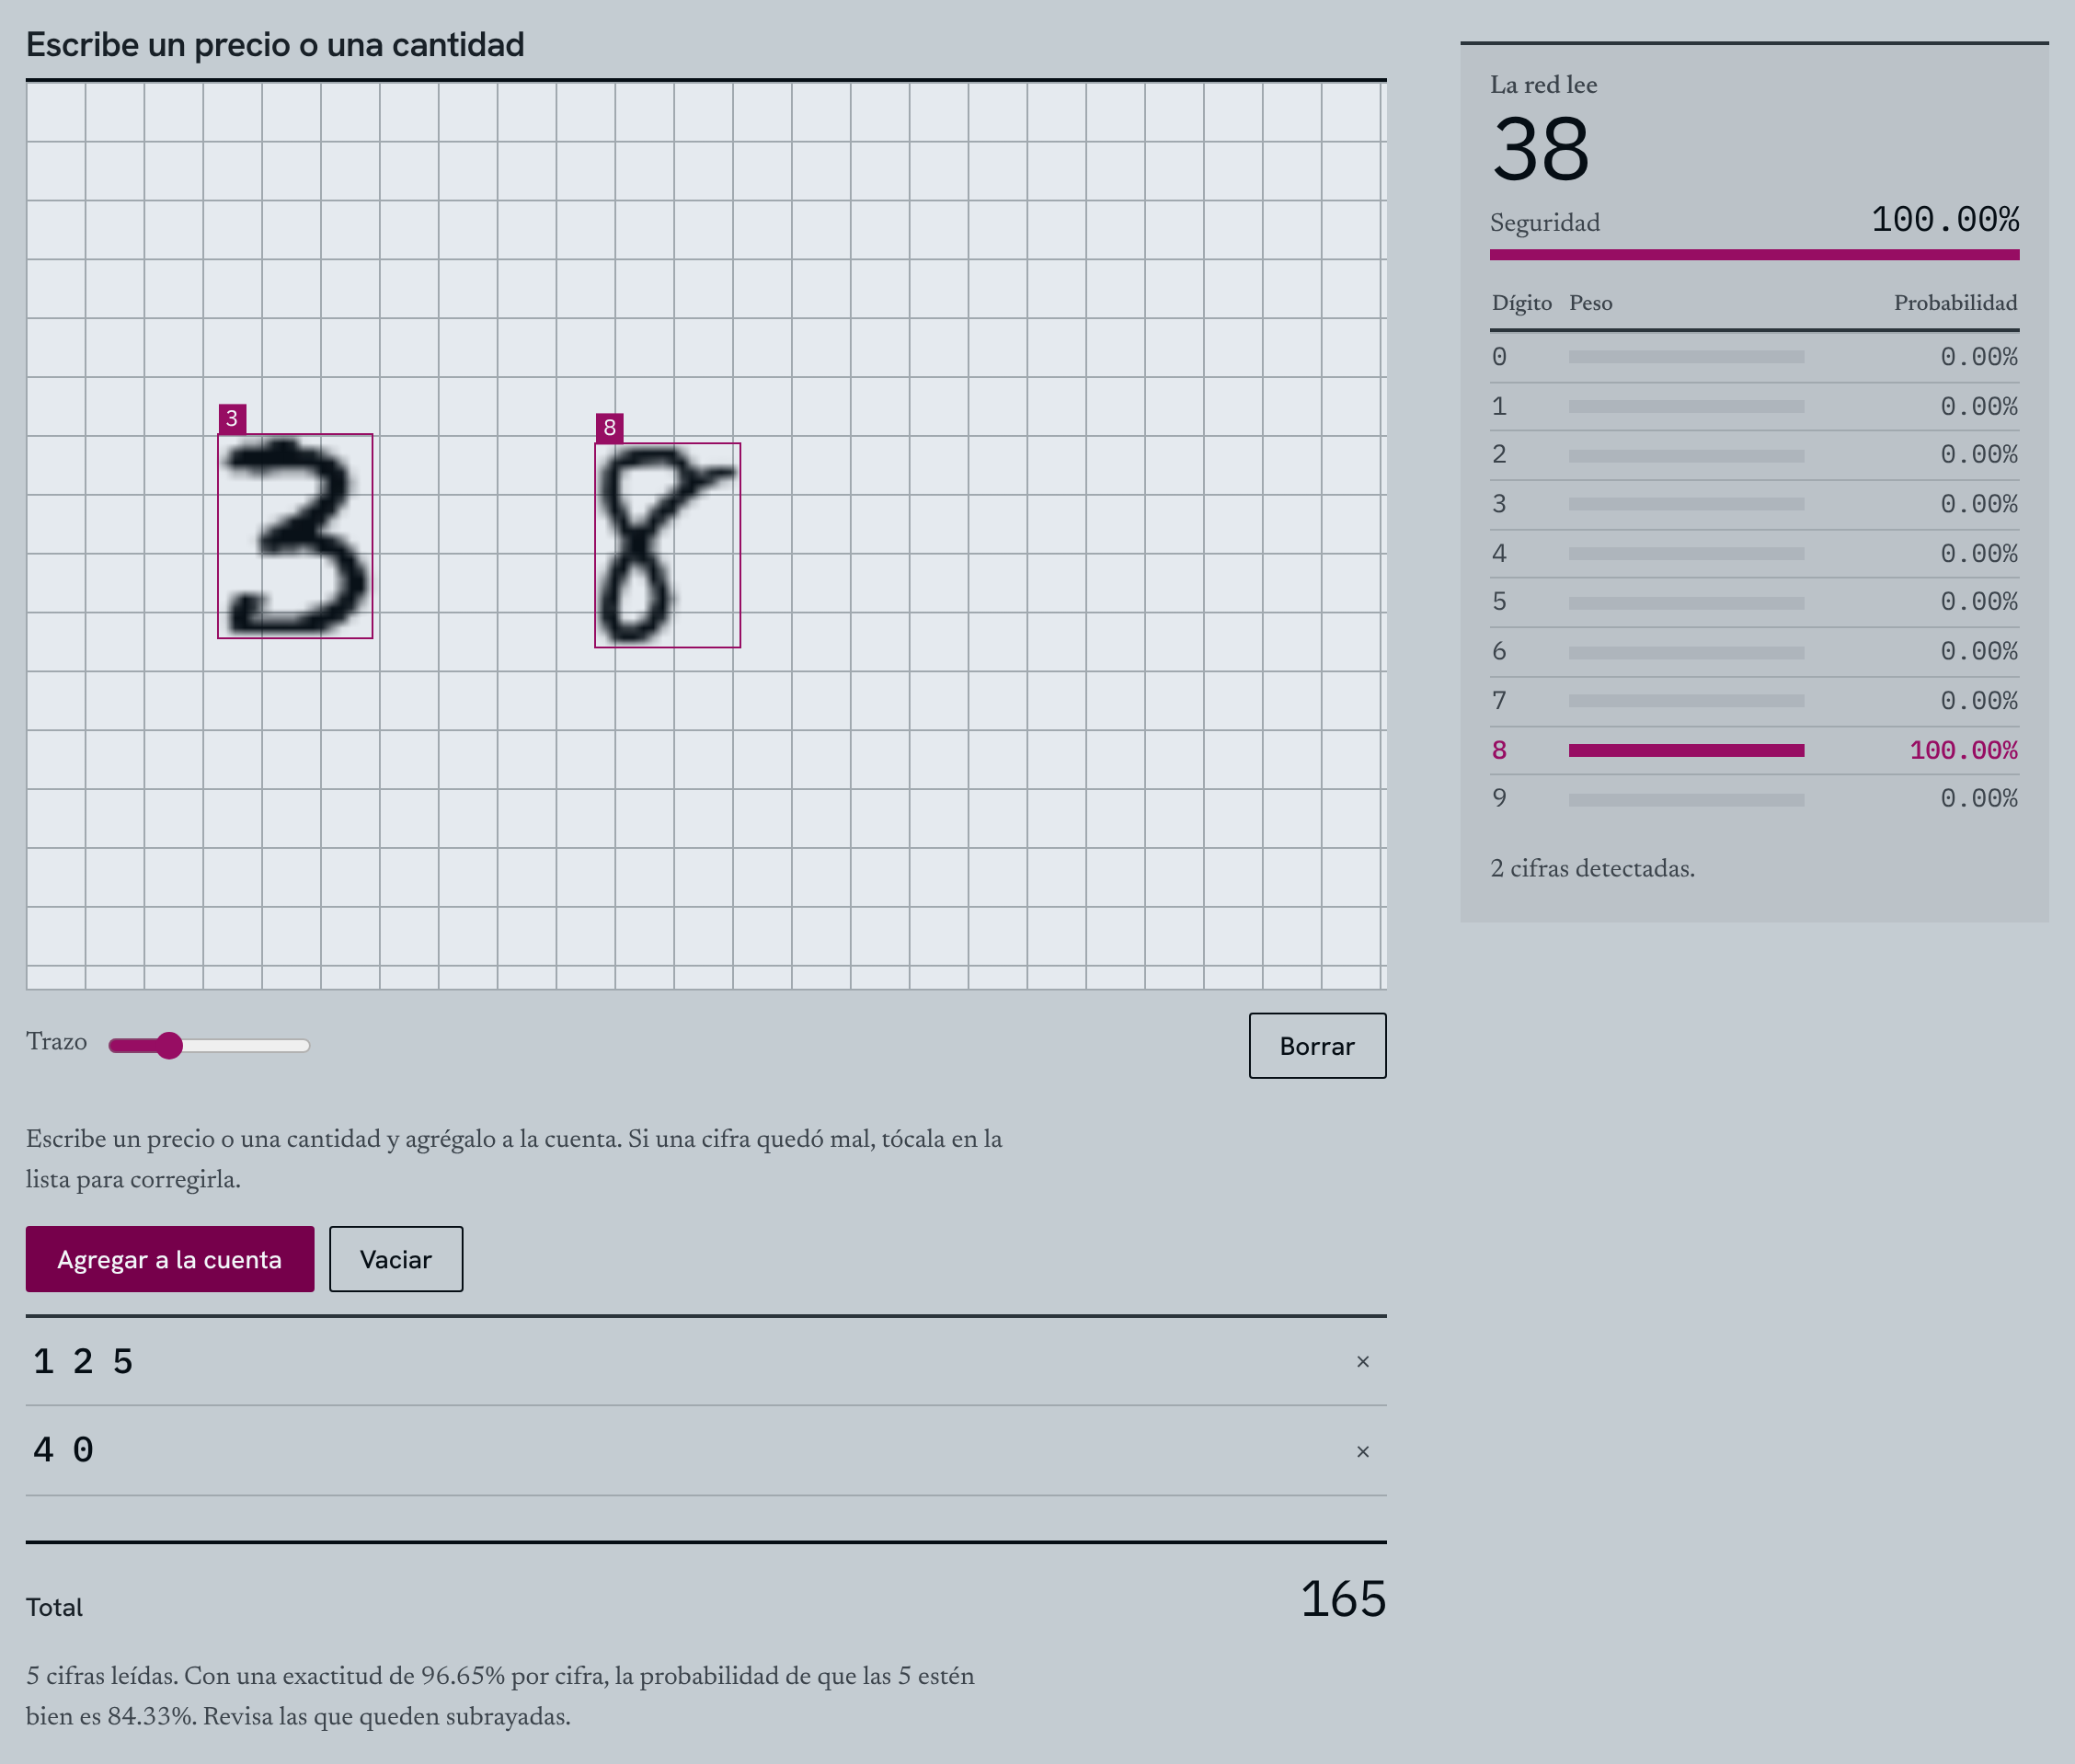
\includegraphics[width=\linewidth]{capturas/app-cuenta.png}
\end{column}
\begin{column}{0.50\textwidth}
\vspace{0.3cm}
Cada cifra se detecta por separado y se encierra en su caja. La red da una
probabilidad a cada uno de los diez dígitos.\par\medskip
Si una cifra queda dudosa, se toca y se corrige. El total se va sumando.\par\medskip
{\color{regla}\rule{\linewidth}{0.6pt}}\par\medskip
{\small\color{apagado}Página web estática, sin servidor.
\textbf{\color{tinta}Ningún dibujo sale del navegador.} Funciona en computador,
celular y tableta, con tema claro y oscuro.}
\end{column}
\end{columns}
\end{frame}
\note{Señalar la caja de cada cifra: eso es lo que después se explica como
separación en componentes conexas.\par\medskip
Abajo a la derecha de la captura dice que con cinco cifras leídas la probabilidad
de que TODAS estén bien es 84.33\,\%. Ese número vuelve más adelante.\par\medskip
30 segundos y pasar a la demo.}

% ==================================================================== demo ===
\begin{oscura}
\vspace{1.2cm}
{\footnotesize\bfseries\color{acentoclaro}AHORA}\par
\vspace{0.4cm}
{\Huge\bfseries\color{claro}Demostración en vivo}\par
\vspace{0.6cm}
{\color{regla}\rule{\textwidth}{0.6pt}}\par
\vspace{0.5cm}
{\large\color{claro}\ttfamily https://szelaya08.github.io/Cifra/}\par
\vspace{0.45cm}
{\normalsize\color{claroapagado}\ttfamily Código: https://github.com/SZelaya08/Cifra}
\end{oscura}
\note{CAMBIAR A LA APP ACÁ.\par\medskip
Guion, máximo dos minutos:\par
1. Modo Práctica: escribir el número que pide. Mostrar que acierta.\par
2. Modo Cuenta: un precio de tres cifras, agregarlo; otro más; mostrar el total.\par
3. Escribir un 4 cerrado a propósito, para que lo lea como 9. Decir: «los errores
no son al azar, y más adelante muestro por qué justo este».\par
4. Abrir «Ver la red por dentro» y dejarlo abierto.\par\medskip
SI FALLA EL WIFI: abrir Cifra-un-solo-archivo.html con doble clic. Es la app
completa en un archivo, funciona sin internet. Tenerlo descargado antes.}

% ================================================================ discreta ===
\section{Matemática discreta}

\begin{frame}{El dibujo \emph{es} una matriz binaria}
\begin{columns}[T]
\begin{column}{0.40\textwidth}
\vspace{0.15cm}
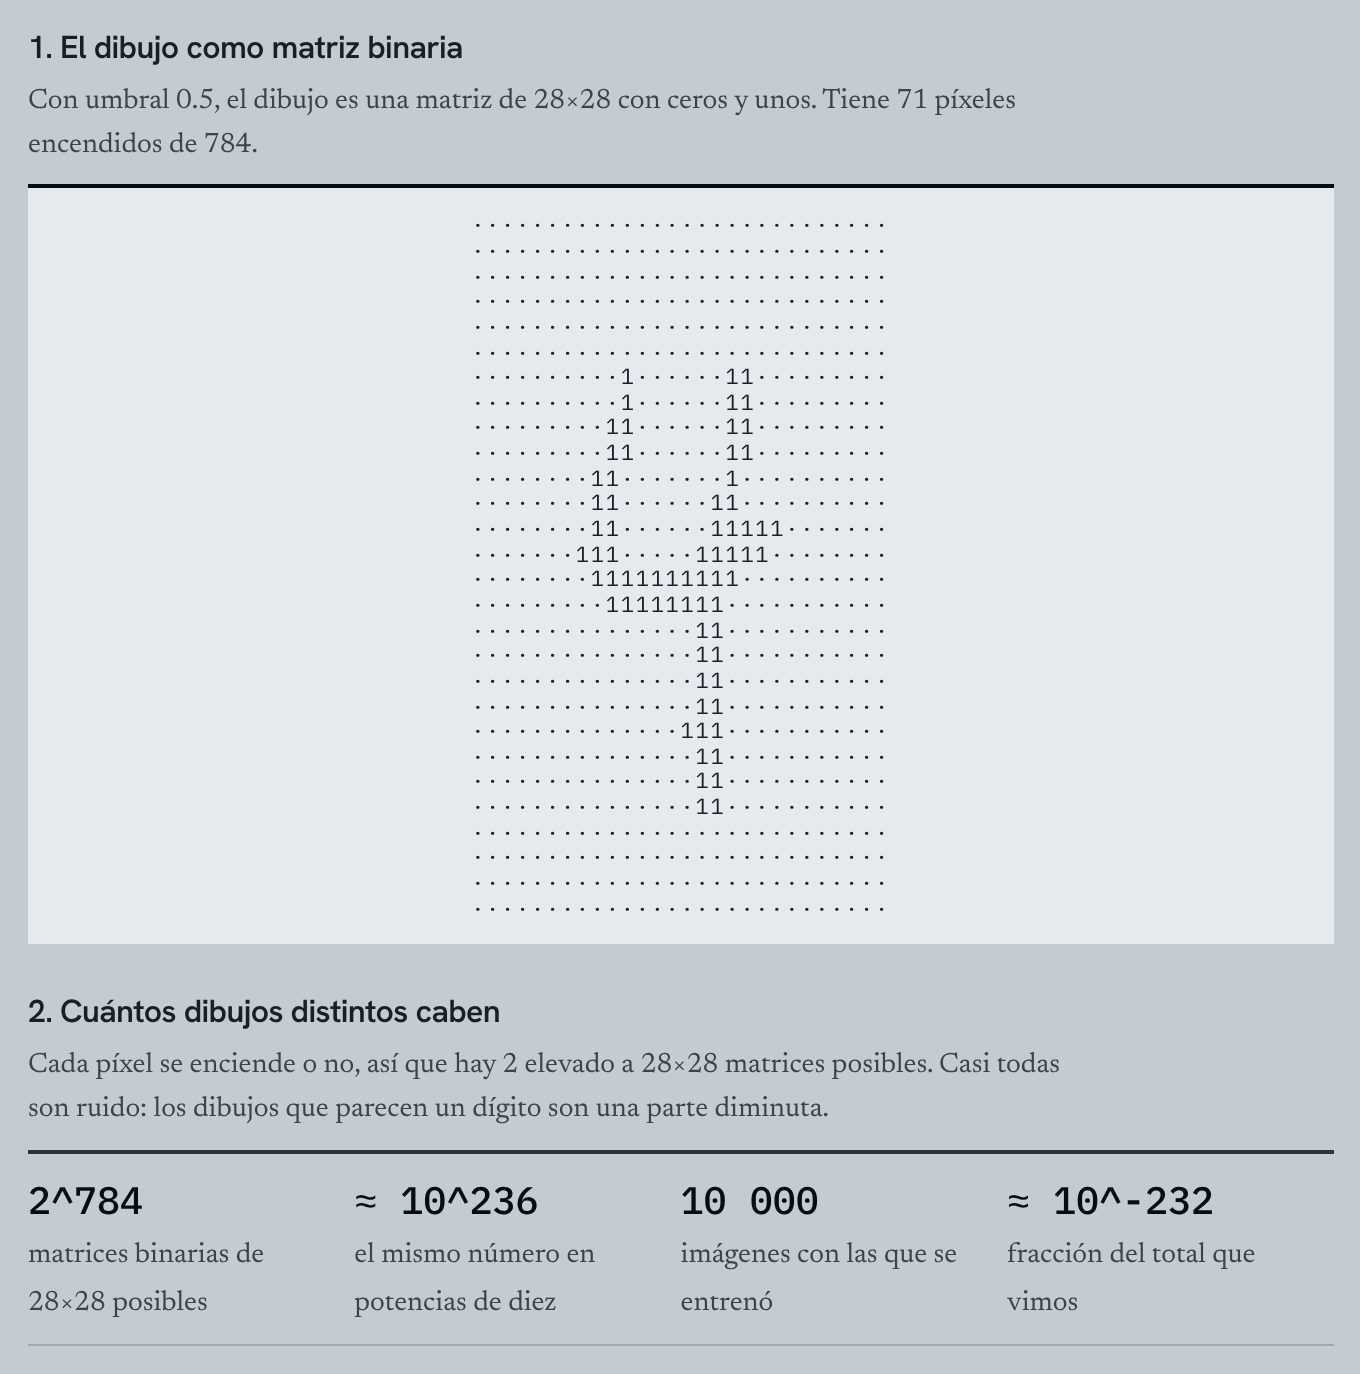
\includegraphics[width=\linewidth]{capturas/panel-discreta-matriz.png}
\end{column}
\begin{column}{0.56\textwidth}
\vspace{0.25cm}
El lienzo se reduce a \textbf{$28\times28 = 784$} píxeles. Con un umbral de
$0.5$, cada uno vale \texttt{0} o \texttt{1}.\par\medskip
Así el dibujo es tres cosas a la vez, y las tres sirven:
\begin{itemize}
\item una matriz booleana de $28\times28$
\item un vector de 784 bits
\item un \textbf{subconjunto} de una retícula de 784 celdas
\end{itemize}
\medskip
{\small\color{apagado}La tercera lectura es la que hace que las operaciones entre
conjuntos tengan sentido inmediato sobre dos dibujos.}
\end{column}
\end{columns}
\end{frame}
\note{«Lo primero que hacemos es dejar de ver un dibujo y empezar a ver una matriz.
Reducimos el lienzo a 28 por 28, o sea 784 casillas, y a cada casilla le ponemos 1
si tiene tinta y 0 si no. Eso que ven ahí son los unos y ceros de verdad del dibujo
que acabo de hacer.»\par\medskip
«Y una vez es una matriz de ceros y unos, también es un vector de 784 bits, y
también es un subconjunto: el conjunto de las casillas encendidas. Esa última forma
de verlo es la que nos deja usar unión, intersección y diferencia entre dos dibujos.»
\par\medskip
Si preguntan por el umbral 0.5: arriba de la mitad de intensidad cuenta como tinta.\par
Si preguntan por qué 28×28: es el tamaño de los datos con que entrenamos, y está
medido que el cuello de botella eran los datos, no la resolución.}

\begin{frame}{Operaciones booleanas entre un 3 y un 8}
\begin{center}
\colorbox{white}{\includegraphics[width=0.80\textwidth]{figuras/booleanas.pdf}}
\end{center}
\vspace{0.1cm}
\begin{columns}[t]
\begin{column}{0.31\textwidth}\tarjeta{\cifra{76}}{píxeles en $3 \wedge 8$\\el trazo que comparten}\end{column}
\begin{column}{0.31\textwidth}\tarjeta{\cifra{184}}{píxeles en $3 \vee 8$\\la unión de los dos}\end{column}
\begin{column}{0.31\textwidth}\tarjeta[fondo]{\cifrac{108}}{\color{claroapagado}píxeles en $3 \oplus 8$\\en cuántos difieren}\end{column}
\end{columns}
\end{frame}
\note{«Si dos dibujos son conjuntos de casillas encendidas, las operaciones de
conjuntos funcionan tal cual. La conjunción deja solo el trazo que comparten. La
disyunción, todo lo que esté en alguno de los dos. Y la disyunción exclusiva,
exactamente las casillas donde uno tiene tinta y el otro no.»\par\medskip
«Fíjense en el último número, 108. Ese es el que importa, porque es el puente a lo
siguiente.» — es literalmente la distancia de Hamming.\par\medskip
Si preguntan de dónde salen el 3 y el 8: son la primera imagen de cada dígito en el
conjunto de entrenamiento, no están escogidas a dedo.\par
Índice de Jaccard: 76 sobre 184, o sea 0.41.}

\begin{frame}{La distancia de Hamming son los unos del XOR}
\begin{center}
\colorbox{white}{\includegraphics[width=0.88\textwidth]{figuras/hamming-deck.pdf}}
\end{center}
\vspace{0.1cm}
{\footnotesize Sobre 1500 imágenes de entrenamiento. Media dentro de una clase
\textbf{111.33} · entre clases distintas \textbf{138.33} · mínima entre dígitos
distintos \textbf{28}}
\end{frame}
\note{LA MÁS IMPORTANTE DE LA PARTE MATEMÁTICA.\par\medskip
«La distancia de Hamming entre dos vectores de bits es en cuántas posiciones
difieren. O sea, contar los unos del XOR: el mismo 108 de hace un momento. Es una
métrica de verdad: cumple las tres propiedades.»\par\medskip
«Entonces la pregunta obvia es: ¿basta con eso para distinguir dígitos? Medimos
todas las distancias entre 1500 imágenes.»\par\medskip
«Y la respuesta es: casi. Las medias sí se separan — 111 dentro de un mismo dígito
contra 138 entre dígitos distintos. Pero miren las colas: se superponen casi
completo. Hay pares de dígitos DISTINTOS a 28 píxeles, muy por debajo de lo que
separa en promedio a dos dibujos del MISMO dígito.»\par\medskip
«Ese traslape, en una sola cifra, es la razón de que necesitemos una red y no solo
una regla geométrica.»\par\medskip
SI TE PIERDES: «contar píxeles distintos funciona sorprendentemente bien, pero no
alcanza, y acá está medido por qué».}

\begin{oscura}
\vspace{0.5cm}
{\footnotesize\bfseries\color{acentoclaro}CARDINALIDAD}\par
\vspace{0.4cm}
{\fontsize{44}{48}\selectfont\bfseries\ttfamily\color{acentoclaro}$2^{784}$}\par
\vspace{0.4cm}
{\large\color{claro}dibujos distintos caben en una retícula de $28\times28$. Por el
principio de la multiplicación: 784 píxeles, dos valores cada uno.}\par
\vspace{0.5cm}
{\color{regla}\rule{\textwidth}{0.6pt}}\par
\vspace{0.45cm}
\begin{columns}[t]
\begin{column}{0.31\textwidth}\tarjeta[fondo2]{\cifrac{237}}{\color{claroapagado}cifras decimales tiene ese número}\end{column}
\begin{column}{0.31\textwidth}\tarjeta[fondo2]{\cifrac{10\,000}}{\color{claroapagado}imágenes tenemos para entrenar y evaluar}\end{column}
\begin{column}{0.31\textwidth}\tarjeta[fondo2]{\cifrac{$10^{-232}$}}{\color{claroapagado}la fracción del espacio que alcanzamos a ver}\end{column}
\end{columns}
\end{oscura}
\note{La más fácil de las cuatro y la que más impresiona.\par\medskip
«¿Cuántos dibujos distintos existen? Cada una de las 784 casillas puede ser 0 o 1,
y las elecciones son independientes, así que por el principio de la multiplicación
son 2 elevado a 784. Ese número tiene 237 cifras.»\par\medskip
«Nosotros tenemos diez mil imágenes. O sea que vimos una fracción de 10 a la menos
232 de todo el espacio.»\par\medskip
REMATE, decirlo completo: «la red TIENE que acertar en dibujos que nunca vio y que
nadie va a ver nunca, porque casi todas esas matrices son ruido sin forma.
Generalizar no es una comodidad del método, es la única salida.»\par\medskip
Si preguntan cómo se sabe que son 237 cifras: el logaritmo en base 10 de 2 elevado
a 784 es 784 por 0.301, que da 236 con algo; el número de cifras es ese más uno.}

\begin{frame}{Por qué una sola capa no basta}
\begin{columns}[T]
\begin{column}{0.40\textwidth}
\vspace{0.3cm}
\centering
\begin{tabular}{ccccc}
\toprule
$p$ & $q$ & $p \wedge q$ & $p \vee q$ & $p \oplus q$ \\
\midrule
0 & 0 & 0 & 0 & 0 \\
0 & 1 & 0 & 1 & 1 \\
1 & 0 & 0 & 1 & 1 \\
1 & 1 & 1 & 1 & 0 \\
\bottomrule
\end{tabular}
\par\medskip
{\footnotesize\color{apagado}\raggedright De las \textbf{\color{tinta}16} funciones
booleanas de dos variables, \textbf{\color{tinta}14} son linealmente separables.
Las dos que no: XOR y XNOR.\par}
\end{column}
\begin{column}{0.56\textwidth}
\colorbox{white}{\includegraphics[width=0.94\linewidth]{figuras/separabilidad.pdf}}
\end{column}
\end{columns}
\vspace{0.25cm}
Pero $p \oplus q \equiv (p \vee q) \wedge \neg(p \wedge q)$ — y esa composición
\textbf{es} una capa oculta.
\end{frame}
\note{EL ARGUMENTO CENTRAL. Practicarlo dos veces en voz alta.\par\medskip
«Una neurona de umbral con dos entradas calcula una función booleana: suma sus
entradas con pesos y responde según si pasa el umbral. Geométricamente eso es trazar
una recta y mirar de qué lado cae el punto.»\par\medskip
«Para AND basta una recta: dejo el (1,1) de un lado y los otros tres del otro.»
\par\medskip
«Para XOR no hay ninguna. Miren la tabla: los dos casos verdaderos son (0,1) y
(1,0), que quedan en una diagonal del cuadrado, y los dos falsos en la otra. Ninguna
recta separa una diagonal de la otra.»\par\medskip
«Entonces, ¿cómo se hace XOR? Componiendo: XOR es la disyunción Y la negación de la
conjunción. Una primera capa calcula OR y NAND, y una segunda neurona los conjuga.
Esa primera capa ES la capa oculta.»\par\medskip
CIERRE: «en la siguiente diapositiva van a ver cuánto cuesta no tener capa oculta:
6.20 puntos.»\par\medskip
Si preguntan cómo verificaron las 14: entrenamos un perceptrón de umbral sobre cada
una de las 16 tablas de verdad. Está en codigo/discreta.py.}

% ============================================================== resultados ===
\section{Resultados}

\begin{frame}{Cuatro modelos, el mismo conjunto de prueba}
\vspace{0.4cm}
\begin{columns}[t]
\begin{column}{0.23\textwidth}\tarjeta{\cifra{11.25\pc}}{siempre el más frecuente\\referencia trivial}\end{column}
\begin{column}{0.23\textwidth}\tarjeta{\cifra{86.80\pc}}{vecino en Hamming\\discreto, sin aprender}\end{column}
\begin{column}{0.23\textwidth}\tarjeta{\cifra{90.45\pc}}{regresión logística\\lineal, sin capas ocultas}\end{column}
\begin{column}{0.23\textwidth}\tarjeta[fondo]{\cifrac{96.65\pc}}{\color{claroapagado}red 784-128-48-10\\dos capas ocultas}\end{column}
\end{columns}
\vspace{0.55cm}
{\color{regla}\rule{\textwidth}{0.6pt}}\par
\vspace{0.4cm}
Lo que importa no es el $96.65\pc$, sino las distancias:
\textbf{+75.55} los da contar píxeles distintos, \textbf{+3.65} aprender cuáles
importan, y \textbf{+6.20} poder combinarlos — lo que una sola capa no puede hacer.
\end{frame}
\note{«Evaluamos cuatro modelos sobre las mismas 2000 imágenes que ninguno vio al
entrenar. Pero el resultado no es el 96.65. Son las distancias entre los cuatro,
porque cada salto se explica con algo distinto.»\par\medskip
Señalar cada salto:\par
· 11.25 a 86.80 son 75.55 puntos, y los da una idea puramente discreta: contar en
cuántas posiciones difieren dos matrices binarias. Sin aprender nada.\par
· 86.80 a 90.45 son 3.65 puntos: aprender qué píxeles importan.\par
· 90.45 a 96.65 son 6.20 puntos: poder combinar trazos parciales. Es el XOR de la
diapositiva anterior, medido en este problema.\par\medskip
«O sea que lo de XOR no era un adorno teórico: 6.20 puntos es el precio de no tener
capa oculta.»\par\medskip
Restas: 86.80−11.25=75.55 · 90.45−86.80=3.65 · 96.65−90.45=6.20 · 96.65−86.80=9.85.\par
Por qué 11.25 y no 10: la clase más frecuente en prueba es el 1, con 225 de 2000.}

\begin{frame}{Pesaron más los datos que el tamaño del modelo}
\begin{columns}[T]
\begin{column}{0.57\textwidth}
\vspace{0.25cm}
\colorbox{white}{\includegraphics[width=\linewidth]{figuras/entrenamiento.pdf}}
\par\medskip
{\scriptsize\color{apagado}El eje de la derecha no arranca en cero: las diferencias
son de décimas de punto.}
\end{column}
\begin{column}{0.39\textwidth}
\vspace{0.4cm}
\tarjeta[fondo]{\cifrac{+1.70}}{\color{claroapagado}puntos ganó el aumento de datos: rotaciones, escalas y desplazamientos}
\par\medskip
\tarjeta{\cifra{+0.07}}{puntos ganó duplicar las neuronas de 32 a 64, con los mismos datos}
\end{column}
\end{columns}
\end{frame}
\note{«Probamos diez arquitecturas en dos vueltas. Ojo con el eje de la derecha: no
arranca en cero, porque las diferencias son de décimas de punto.»\par\medskip
«Y acá hay un resultado que no esperábamos. Duplicar las neuronas, de 32 a 64,
mejoró 0.07 puntos. Nada. En cambio generar variantes de las imágenes — rotarlas un
poco, cambiarles el tamaño, correrlas — mejoró 1.70 puntos.»\par\medskip
«O sea que nuestra limitación no era la capacidad del modelo sino la cantidad y
variedad de los datos. Usamos 10\,000 de las 70\,000 que tiene MNIST.»\par\medskip
La arquitectura 32-16 aparece dos veces a propósito: comparar sus dos puntos aísla
el efecto del aumento de datos sin cambiar nada más.\par\medskip
Red final, por si lo piden: 107\,162 parámetros, ReLU y softmax, entropía cruzada,
optimizador Adam, tasa inicial 0.003, lotes de 256, 32 iteraciones. Entrenamiento
99.70\,\% contra prueba 96.65\,\%: sobreajuste moderado, declarado.}

\begin{frame}{Los errores no se reparten al azar}
\begin{columns}[T]
\begin{column}{0.40\textwidth}
\vspace{0.15cm}
\colorbox{white}{\includegraphics[width=\linewidth]{figuras/confusion.pdf}}
\end{column}
\begin{column}{0.56\textwidth}
\vspace{0.4cm}
\centering
\begin{tabular}{ccc}
\toprule
\textbf{Dígito real} & \textbf{Leído como} & \textbf{Casos} \\
\midrule
4 & 9 & 7 \\
2 & 7 & 5 \\
5 & 3 & 5 \\
8 & 6 & 4 \\
\bottomrule
\end{tabular}
\par\medskip
\raggedright\small
Todos son pares que \textbf{comparten trazo}. Si el trazo de arriba del 4 se
cierra, lo que queda es un 9.\par\medskip
{\color{apagado}La red se equivoca donde se equivocaría una persona apurada, no en
cualquier parte.}
\end{column}
\end{columns}
\end{frame}
\note{«Acá está la matriz de confusión completa. La diagonal son los aciertos; todo
lo de afuera son errores, y son poquitos.»\par\medskip
«Lo interesante es que no están repartidos al azar. Los cuatro pares más confundidos
comparten trazo. El más frecuente es 4 leído como 9, siete casos, y es el que uno
esperaría: si el trazo de arriba del 4 se cierra, la figura que queda es un 9.»
\par\medskip
«Dicho de otro modo: la red se equivoca donde se equivocaría una persona apurada.»
\par\medskip
Si se hizo el 4 cerrado en la demo, amarrarlo acá.\par
Dígito más difícil: el 2 y el 4 por exhaustividad; los mejores, el 1 y el 0. La
tabla completa por dígito está en el anexo C del informe.}

\begin{oscura}
\vspace{0.25cm}
{\footnotesize\bfseries\color{acentoclaro}LO QUE CAMBIÓ EL DISEÑO}\par
\vspace{0.2cm}
{\LARGE\bfseries\color{claro}Un precio de cuatro cifras falla uno de cada ocho}\par
\vspace{0.55cm}
\begin{columns}[T]
\begin{column}{0.42\textwidth}
\centering
{\color{claro}
\begin{tabular}{cc}
\toprule
\textbf{Cifras} & \textbf{Se lee bien completo} \\
\midrule
1 & $96.65\pc$ \\
2 & $93.41\pc$ \\
3 & $90.28\pc$ \\
4 & $87.25\pc$ \\
5 & $84.33\pc$ \\
\bottomrule
\end{tabular}}
\end{column}
\begin{column}{0.54\textwidth}
{\fontsize{30}{34}\selectfont\bfseries\ttfamily\color{acentoclaro}$0.9665^{\,k}$}\par
\vspace{0.4cm}
{\color{claro}Todas las cifras tienen que acertarse \textbf{a la vez}. Una exactitud
por cifra que suena alta se vuelve frágil en un número largo.}\par
\vspace{0.3cm}
{\small\color{claroapagado}Por eso el modo de cuenta no muestra solo el total:
muestra \textbf{\color{claro}cada cifra por separado} y deja corregirla con un toque.}
\end{column}
\end{columns}
\end{oscura}
\note{La que más les gusta a los jurados, porque es honestidad sobre el propio
trabajo.\par\medskip
«Hay una diferencia entre acertar y ser útil. Si la exactitud por cifra es
96.65\,\% y los errores son independientes, la probabilidad de leer bien un número
de k cifras es 0.9665 elevado a k. Para un precio de cuatro cifras eso da
87.25\,\%: falla algo más de uno de cada ocho.»\par\medskip
«Reconocer eso nos cambió el diseño. En vez de mostrar un total y confiar en él, el
modo de cuenta expone cada cifra y deja corregirla. Un sistema honesto sobre su
incertidumbre termina siendo más usable que uno que la esconde.»\par\medskip
VERIFICACIÓN del supuesto de independencia: probamos 100 números de tres cifras. La
separación salió bien en los 100, y el número completo en 89. La teoría predecía
90.28. Cuadra.\par\medskip
Calibración: la app usa umbral 0.80 y marca las cifras por debajo. Se acepta el
98.75\,\% de las lecturas y las aceptadas tienen 97.16\,\% de exactitud.}

\begin{frame}{No muestra el resultado: muestra la cuenta}
\begin{columns}[T]
\begin{column}{0.37\textwidth}
\vspace{0.15cm}
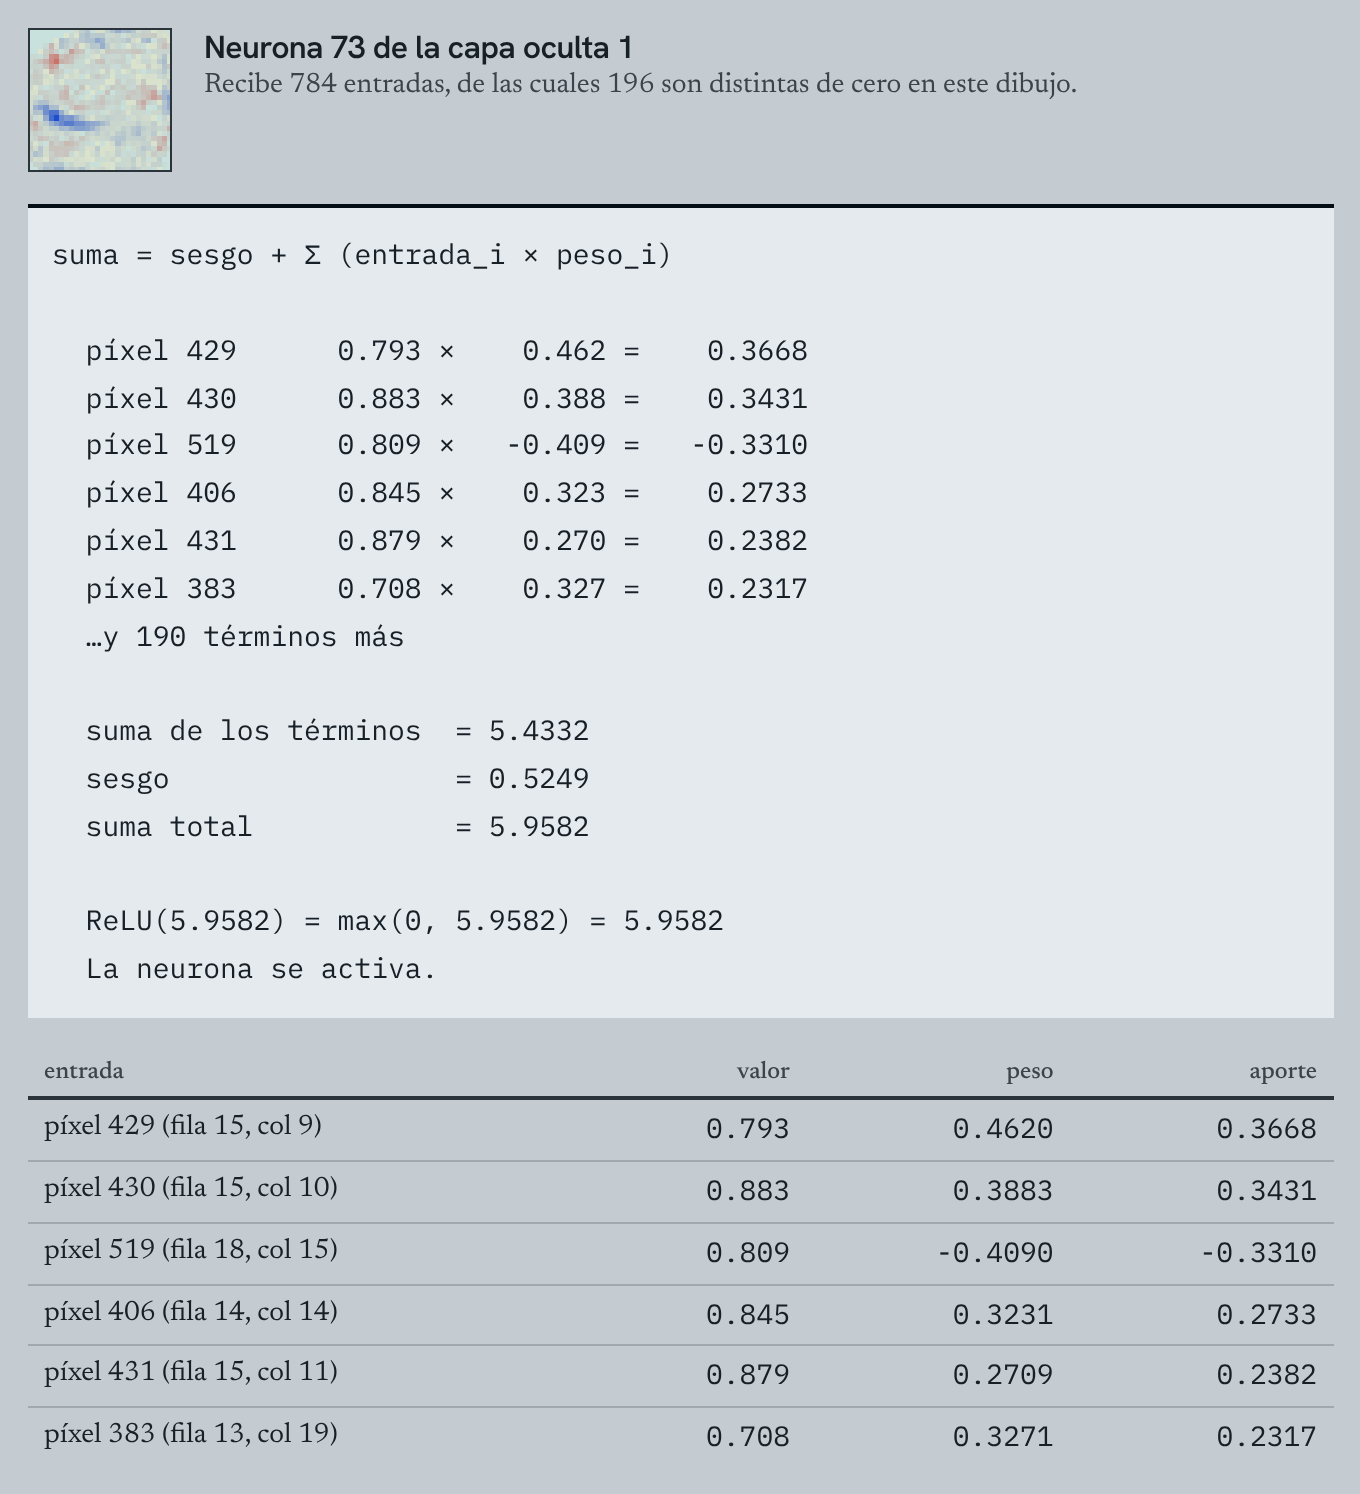
\includegraphics[width=\linewidth]{capturas/panel-calculo.png}
\end{column}
\begin{column}{0.59\textwidth}
\vspace{0.25cm}\small
La red se reescribió a mano en JavaScript, sin librerías, para poder enseñar
cualquier valor interno mientras corre.
\begin{itemize}
\item \textbf{Capas} — cada neurona encendida según el dibujo
\item \textbf{Neuronas} — los pesos vistos como imagen de $28\times28$
\item \textbf{Cálculo} — la suma ponderada, término a término
\item \textbf{Discreta} — matriz binaria, conteo del espacio y Hamming
\item \textbf{Entrenar} — reentrenar con tus propios trazos
\end{itemize}
\medskip
{\color{regla}\rule{\linewidth}{0.6pt}}\par\medskip
{\color{apagado}Verificado contra la versión de Python: las \texttt{20} clases
coinciden, con diferencia máxima de \texttt{0.000016} en probabilidad.}
\end{column}
\end{columns}
\end{frame}
\note{«Esto es lo que convierte el proyecto en un instrumento de explicación y no
solo en un clasificador. Lo que ven ahí no es un ejemplo ilustrativo: son los
números que la red está usando en este momento con el dibujo que hay en pantalla.»
\par\medskip
Se puede volver a la app acá en vez de mostrar la captura. Es más contundente.
\par\medskip
Sobre la diferencia de 0.000016: no es un error. Python calcula en doble precisión y
el navegador en precisión simple. El criterio fue que la clase predicha coincida
siempre y las probabilidades puedan diferir hasta 0.0001.\par\medskip
Reentrenamiento: es una demostración del mecanismo, no un entrenamiento serio.
Mezclamos los dibujos nuevos con 300 imágenes de referencia para evitar el olvido
catastrófico.}

% ================================================================== cierre ===
\section{Cierre}

\begin{frame}{Lo que declaramos como limitación}
\vspace{0.3cm}
\begin{columns}[T]
\begin{column}{0.47\textwidth}
\begin{itemize}\small
\item Los datos son dígitos escritos \textbf{con lápiz} por adultos
  estadounidenses. Un trazo de dedo es distinto: la exactitud real de uso puede ser
  menor que $96.65\pc$.
\item Usamos \textbf{10\,000 de las 70\,000} imágenes de MNIST.
\item No se ha probado con usuarios reales escribiendo con el dedo, ni con niños ni
  con comerciantes.
\end{itemize}
\end{column}
\begin{column}{0.47\textwidth}
\begin{itemize}\small
\item El panel muestra lo que la red \textbf{hace}, no lo que entiende. Leer los
  pesos de una neurona no es una afirmación sobre lo que representa.
\item \textbf{Ocho de las 128} neuronas de la primera capa nunca se activan. La
  arquitectura tiene holgura.
\item Los signos $+\ -\ \times\ =$ quedaron fuera: hacía falta recolectar muestras
  propias de cada uno.
\end{itemize}
\end{column}
\end{columns}
\end{frame}
\note{DECIRLAS ANTES DE QUE LAS PREGUNTEN. Un jurado que ve que ya las
identificaste deja de buscarlas.\par\medskip
La de las neuronas muertas es la que más puede sorprender: «son neuronas cuya suma
ponderada queda negativa para toda entrada; la ReLU les devuelve cero siempre y
dejan de recibir gradiente, así que se quedan con los pesos aleatorios del inicio.
La red usa 120 de sus 128. Tengo la imagen de respaldo.»\par\medskip
No es un error: es un efecto conocido de ReLU y no afecta el resultado medido.
Indica que la arquitectura podría ser algo menor sin perder exactitud.\par\medskip
Por qué 10\,000 y no 70\,000: los sitios oficiales de MNIST no eran alcanzables
desde donde trabajamos, y el paquete de npm que usamos trae 10\,000 incluidas.}

\begin{oscura}
\vspace{0.8cm}
{\footnotesize\bfseries\color{acentoclaro}CONCLUSIONES}\par
\vspace{0.5cm}
{\large\color{claro}El problema se deja formular \textbf{entero} en matemática
discreta: matriz binaria, operaciones booleanas, distancia de Hamming, cardinalidad
$2^{784}$ y una relación de equivalencia que lo parte en diez clases.}\par
\vspace{0.4cm}
{\color{regla}\rule{\textwidth}{0.6pt}}\par
\vspace{0.4cm}
{\large\color{claro}La necesidad de capas ocultas quedó justificada dos veces y de
forma concordante: \textbf{teórica}, porque XOR no es linealmente separable, y
\textbf{empírica}, porque el modelo sin capas ocultas se queda $6.20$ puntos abajo.}\par
\vspace{0.4cm}
{\color{regla}\rule{\textwidth}{0.6pt}}\par
\vspace{0.4cm}
{\large\color{claro}Y la red no se quedó en un clasificador: corre en el navegador,
verificada contra Python, enseñando su propio cálculo \textbf{mientras trabaja}.}\par
\vspace{0.3cm}
{\footnotesize\color{claroapagado}\ttfamily https://github.com/SZelaya08/Cifra \quad·\quad https://szelaya08.github.io/Cifra/}
\end{oscura}
\note{Tres frases, sin leer la diapositiva:\par\medskip
«Para cerrar: el problema se deja describir entero con lo que vimos en el curso. No
es que le hayamos puesto matemática discreta encima a un proyecto de redes
neuronales; es que el problema ya era discreto.»\par\medskip
«La necesidad de capas ocultas la justificamos dos veces por caminos distintos y las
dos concuerdan: por XOR, que no es linealmente separable, y midiendo, que son 6.20
puntos.»\par\medskip
«Y lo que más nos interesaba: la red no se quedó en un clasificador. Corre en el
navegador enseñando su propio cálculo mientras trabaja.»\par\medskip
«Gracias — quedamos atentos a preguntas.»\par\medskip
Después vienen las diapositivas de respaldo. No pasarlas; dejarlas para preguntas.}

% ================================================================ respaldo ===
\section{Respaldo}

\begin{oscura}
\vspace{1.4cm}
{\footnotesize\bfseries\color{acentoclaro}PARA PREGUNTAS}\par
\vspace{0.4cm}
{\Huge\bfseries\color{claro}Respaldo}\par
\vspace{0.5cm}
{\color{regla}\rule{\textwidth}{0.6pt}}\par
\vspace{0.5cm}
{\small\color{claroapagado}Los pesos de las neuronas y las ocho que nunca se activan
\quad·\quad Por qué los pesos no se parecen al dígito \quad·\quad El preprocesado
del trazo y lo que cuesta}
\end{oscura}
\note{No pasar de acá en la exposición normal. Solo para preguntas.}

\begin{frame}{Ninguna neurona se parece a un dígito}
\vspace{0.25cm}
\begin{center}
\colorbox{white}{\includegraphics[width=0.94\textwidth]{figuras/neuronas-deck.pdf}}
\end{center}
\vspace{0.1cm}
{\footnotesize Rojo suma, azul resta. Las recuadradas, \textbf{n9} y \textbf{n27},
son neuronas muertas: conservan el ruido de su inicialización porque nunca llegaron
a activarse.}
\par\medskip
\small Cada cuadro son los pesos de \textbf{una} neurona. Ninguna se parece a un
dígito: cada una responde a un \textbf{trazo parcial}, y es la segunda capa la que
los combina.
\end{frame}
\note{Para cuando pregunten «¿y qué aprendió cada neurona?».\par\medskip
«Cada cuadrito son los pesos de una neurona de la primera capa, vistos como imagen
de 28 por 28. El rojo suma y el azul resta: la neurona se activa cuando el trazo cae
sobre el rojo y evita el azul.»\par\medskip
«Ninguna se parece a un dígito. Cada una responde a un trazo parcial, y es la
segunda capa la que los combina. Eso es el XOR otra vez.»\par\medskip
Las dos recuadradas son las neuronas muertas. Son 8 de 128 en total; acá se ven las
primeras 32.\par\medskip
CUIDADO con decir que una neurona «detecta» algo concreto: es una lectura de sus
pesos, no una afirmación sobre lo que representa. Está declarado como limitación.}

\begin{frame}{Los pesos no son un retrato del dígito}
\vspace{0.35cm}
\begin{center}
\colorbox{white}{\includegraphics[width=0.92\textwidth]{figuras/plantillas.pdf}}
\end{center}
\vspace{0.1cm}
{\footnotesize Arriba, la imagen promedio de cada dígito. Abajo, los pesos que
aprende la regresión logística sin capas ocultas para ese mismo dígito.}
\par\medskip
\small Los pesos no describen \textbf{cómo es} el dígito, sino \textbf{qué lo
distingue} de los otros nueve. Por eso se ven revueltos, y por eso la imagen
promedio —que sí parece un dígito— no sirve para clasificar.
\end{frame}
\note{Para cuando pregunten «¿pero no deberían verse como el número?». Es la
pregunta más común.\par\medskip
«Es tentador esperarlo, pero no pasa, ni siquiera en un modelo de una sola capa.
Arriba está la imagen promedio de cada dígito, que sí parece un dígito. Abajo, los
pesos que ese mismo modelo aprende, que se ven revueltos.»\par\medskip
«La razón es que los pesos no describen cómo ES el dígito, sino qué lo DISTINGUE de
los otros nueve.»\par\medskip
DATO BUENO para cerrar: intentamos suavizar los pesos subiendo la regularización, a
ver si se veían más como dígitos. La textura casi no cambió y la exactitud cayó de
90.45\,\% a 81.35\,\%. Preferimos explicar el fenómeno antes que forzar la imagen.}

\begin{frame}{El preprocesado fue la pieza crítica}
\begin{columns}[T]
\begin{column}{0.54\textwidth}
\vspace{0.3cm}\small
En los datos, cada dígito viene recortado, escalado a una caja de
$20\times20$ y centrado por su \textbf{centro de masa} dentro del cuadro de
$28\times28$.\par\medskip
Un trazo de dedo sin ese tratamiento le llega a la red como algo que nunca vio. La
app repite la misma cadena: separa trazos en componentes conexas, los junta por
cifra, recorta, escala y centra.\par\medskip
{\color{regla}\rule{\linewidth}{0.6pt}}\par\medskip
{\footnotesize\color{apagado}Medido en los datos: alto medio \texttt{19.68} px ·
ancho medio \texttt{15.59} px · centro de masa en la fila \texttt{13.99} y la
columna \texttt{14.00}}
\end{column}
\begin{column}{0.42\textwidth}
\vspace{0.45cm}
\centering\small
\begin{tabular}{lr}
\toprule
\textbf{Cómo se dibuje} & \textbf{Exactitud} \\
\midrule
Entrada directa & $96.33\pc$ \\
Centrado & $96.00\pc$ \\
Pequeño & $96.00\pc$ \\
En una esquina & $96.00\pc$ \\
Corrido a la derecha & $96.00\pc$ \\
Grande, tocando el borde & $94.00\pc$ \\
\bottomrule
\end{tabular}
\end{column}
\end{columns}
\vspace{0.45cm}
Cuesta \textbf{0.33} puntos y, a cambio, la lectura deja de depender de dónde y de
qué tamaño se escriba.
\end{frame}
\note{Para «¿y si escribo chiquito o en una esquina?» o «¿qué fue lo más difícil?».
\par\medskip
«Este fue el punto donde el proyecto estuvo más cerca de fallar en la práctica. Las
imágenes con que entrenamos no son trazos sueltos: vienen recortadas, escaladas a
una caja de 20 por 20 y centradas por centro de masa. Si le entregáramos el trazo
tal como se dibuja, le llegaría descentrado y con otra escala, y fallaría aunque el
modelo fuera bueno.»\par\medskip
«Así que la app repite exactamente la misma cadena. Cuesta 0.33 puntos de exactitud
y, a cambio, da casi igual dónde y de qué tamaño escribas. Lo único que pierde algo
es dibujar muy grande, porque el trazo toca el borde y el recorte pierde parte de la
figura.»\par\medskip
Engrosado: las imágenes de entrenamiento tienen en promedio 103.97 píxeles
encendidos. Si alguien dibuja con trazo muy fino, al encoger quedan muchos menos.
Cuando baja de 48, la app engrosa el trazo. Es una corrección del preprocesado, no
del modelo.}

\end{document}
